\documentclass[jou]{apa6}

\usepackage[american]{babel}

\usepackage{csquotes}
\usepackage[style=apa,sortcites=true,sorting=nyt,backend=biber]{biblatex}
\DeclareLanguageMapping{american}{american-apa}
\addbibresource{bibliography.bib}

\title{Music Composition Assisted by Machine Learning}

\author{Nianze Liu}
\affiliation{New York University}

\leftheader{Liu}

\abstract{This article overviews recent progress in machine learning as a creative assistance in music production. Specifically, two innovative machine learning models, NSynth and Coconet, are introduced and dicussed in the context of music composition, music production, and music live performance.}

\keywords{Computer Music, Machine Learning}

\begin{document}
\maketitle

\section{Introduction}

Since the invention of computer, music industry has hugely been influenced. Nowadays, we can find tons of music pieces in the digital format: some might be played by acoustic instruments and recorded down, others may be generated by synthesizers, but no matter how the sound is generated, the music waves ends up into a sequence of digital representations, which turns out to be a good data source for machine to learn from. With the hardware becomes more and more powerful in the recent years, more complicated machine learning models become feasible for providing helpful assistance in various areas, such as automatic driving and speech recognition. Music production is no exception under this trend. By the help of new machine learning models, we might train the computer to learn the musical master's composition techniques to help generate harmonies given a piece of melody we write; it is also possible to synthesize new sound that might be very difficult to create by the old synthesizer-based motheds.

In this article, two machine learning models are discussed. We will go over their basic structures to see how they work. After understanding the abilities of these innovative models, we will discuss what might be changed by introducing these techniques into the current music composition, music production and even live music performance, and what might be achieved in the future.

\section{Computer Assisted Composition}

\subsection{How Computer Generates Music}

Traditionally, when computer generates music, the most natural way is to do the job in a sequence, under an orderly manner, because when computer generates music, the only thing it understands is just numbers, or in our context, statistics and probability - it does not feel like humans do. Given a note, such as C4, and another note, say E4, the computer has to calculate all the possibilities of the next note, and return the most possible notes to fill in the next position. If the model sees 90 percent of time that C4, E4 and G4 always show together during training, the likelihood of generating a G4 given the context of C4 and E4 is then higher than other options -- this higher possibility is stored in the model in the form of network weight and we can say that the model 'learns' the C major triad now. 

Under this sequential generation process, traditionally, before determining the very first note of music, the computer has to have a complete view of the whole piece of music, since as long as the previous note is determined, there’s no way back to refine it anymore -- the note has to be generated in a sequence in one iteration. This orderly generation requirement is very strict, which leads to the creation of a new machine learning model named 'Coconet'.

\subsection{Coconet}

The machine learning model Coconet is basically a convolutional neural network but is integrated with some creative process. The details of the model are described in \textcite{huang2019counterpoint}. Here we will just go over the basics of the model structure and see how it works to generate four voices counter points and harmonize any given input melody.

The biggest idea behind the model is to mimic the process of human composition. The key observation here is that, when human beings compose, the composer seldom writes the music in sequence. Instead, human composer tends to rewrite the same piece back and forth over and over again in order to get the better refined result that finally meets his or her standard. In other words, the composition is typically done in an orderless manner. To achieve orderless composition by computer, two techniques is created: Orderless modeling & Gibbs sampling.

The basic idea is to use Gibbs sampling to generate music in multiple iterations, and in every iteration, part of music scores is erased, so that we can use Orderless modeling to come up with the independent conditional probabilities for missing notes. For the same example of C4 E4 G4 triad above, if we mask the E4 in the middle, the model should be able to generate E4 given the context of C4 in the first position and G4 in the 3rd position. In math, the model is basically computing: 

\centerline{P($x_2|x_1, x_3$), where $x_n$ means score at beat n}

Since the model doesn't know which note will be erased, in orderless modeling, all possible generation sequences have to be modeled. In the example of 3 notes, there are $3! = 6$ possible permutations.

Gibbs sampling, on the other hand, is just a fancy word for phrasing our repeated iterative music generation/modification in multiple passes, and orderless modeling guarantees that no matter which note is randomly erased by a mask in a random iteration, the model is able to generate a conditional distribution for the missing score. Figure~\ref{fig:Figure1} below shows this multi-iteration music notes generation and erasing during the training phase.

\begin{figure}[h!]
    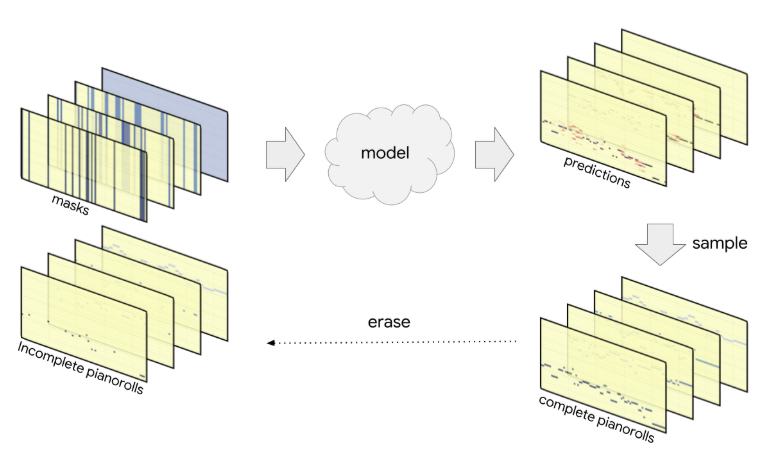
\includegraphics[width=\linewidth]{coconet.png}
    \caption{Music generation in multiple iterations}
    \label{fig:Figure1}
\end{figure}

The result of Coconet is very interesting: given a partial piece of scores for a fixed length, the model is able to complete the music based on how it gets trained. On 2019 March 20, in order to celebrate J.S. Bach's 334th birthday, Google released a Doodle powered by this coconet model, which learns from "a dataset of 306 chorale harmonizations by Bach", according to Magenta Blog post.

\section{Computer Assisted Systhesis}

The output of coconet is abstract music notes, which can not be heard directly and functions similarly to MIDI in that we can use synthesizers to generate different timbre for the generated note. Traditional hardware and software synthesizers generate audio by pre-designed oscillators and wavetables. By taking advantage of machine learning, however, there comes a new way to generate audio: by using deep neural networks to extract multi-dimentional sound representations from training data set, and then applying high level modification over these representations to generate original new sound that could be very hard to generate in the traditional way. The NSynth model introduced in \textcite{engel2017neural} follows this thought and achieves a remarkable result.

\subsection{NSynth}

The basic structure of NSynth, as shown in Figure~\ref{fig:Figure2}, is a fully convolutional neural network, which is pretty similar to the structure of Wavenet introduced in \textcite{oord2016wavenet}.

\begin{figure}[h!]
    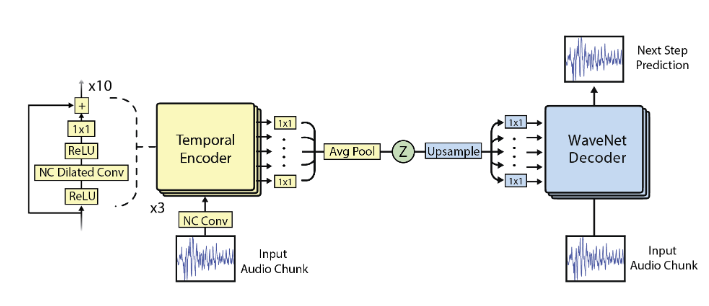
\includegraphics[width=\linewidth]{nsynth.png}
    \caption{Training workflow for NSynth}
    \label{fig:Figure2}
\end{figure}

\section{Future Possibilities}

Combining the two models mentioned above, we can already see some possible future of music production.

\printbibliography

\end{document}